\documentclass[11pt]{article}
\usepackage[utf8]{inputenc} % standard input encoding
\usepackage[T1]{fontenc} % standard modern font encoding
\usepackage{lmodern} % use Latin Modern font (it has vectorized special characters = better copying od searching in pdfs)
\usepackage[czech]{babel}
\usepackage[a4paper]{geometry} % margin adjustment
\usepackage[pdfusetitle]{hyperref} % metadata, content in pdf, hyperlinks
\usepackage{easyReview}

\usepackage{graphicx}
\graphicspath{ {./images/} }

% bibliography
\usepackage[backend=bibtex]{biblatex}
\addbibresource{bibliography.bib}

\def\MainTitle{Automatická detekce ischemické léze z MR obrazových dat u cévní mozkové příhody}
\def\Subtitle{Diplomový projekt}
\date{\large \hfill \today}

\hypersetup{pdftitle={\MainTitle}} % add main title to the pdf metadata
\title{
	\ifdefined\Subtitle \large \Subtitle \\[1em] \fi
	\LARGE \textbf{\MainTitle} \\[2em]
	\begin{large}
	\begin{minipage}{3cm}
		\textbf{Autor:}\\
		Jakub Šmíd
	\end{minipage}
	\hfill
	\begin{minipage}{6cm}
		\textbf{Vedoucí:}\\
		prof. MUDr. Jakub Otáhal, Ph.D. \\
		Ing. David Kala
	\end{minipage}
	\end{large}
}

\begin{document}
\maketitle

\section{Popis projektu}
Cévní mozková příhoda (mrtvice) je jedním z nejčastějších onemocnění a příčin úmrtí celosvětově. Zásadní krok při jejím vyšetření je segmentace poškozené tkáně na obrazech z magnetické resonance. V současné klinické praxi se segmentace provádí manuálním obkreslováním a kvůli tomu je velmi časově náročná a výsledky podléhají značné subjektivitě. Cílem této práce je celý proces zrychlit přidáním prvků automatické segmentace obrazu.
Práce bude probíhat v úzké spolupráci s Fakultní nemocnicí v Motole a neurovědci z EpiReC zabývající se dlouhodobě problematikou cévní mozkové příhody a souvisejících onemocnění.

Téma propojuje technické znalosti (zpracování obrazu, návrh algoritmů) s lékařským prostředím neurověd.

\section{Segmentace}
\section{Evaluační metriky}
Před tím, než se začneme věnovat publikacím a aktuálnímu stavu poznání, je nutné uvést metriky, na základě kterých budeme moci vyhodnotit úspěšnost segmentačních algoritmů. Díky uvedeným metrikám je možné srovnat kvalitu dvou segmentací stejného vzoru - typicky segmentaci experta (radiologa) a automatickou segmentaci.

Pro porovnání dvou segmentací jsou používány následující míry: dice similarity coefficient, average symetric surface distance. Pro vyhodnocení \alert{over- a under-segmentation} se používají metriky známé pod pojmy precision a recall. \cite{Maier2016, Ito2018}
\subsection{Dice similarity coefficient}
Dice similarity coefficient dále označovaný jako DC je mírou přesnosti segmentace.
\begin{equation}
	\label{DC}
	DC = 2 \frac{|A \cap B|}{|A|+|B|}
\end{equation}
Vztah pro výpočet DC je dán rovnicí \ref{DC}, kde A a B jsou dvě poměřované segmentace. DC koeficient nabývá hodnot mezi 0 a 1 a popisuje překryv mezi jednotlivými segmentacemi. Porovnávání dvou různých DC je citlivé na velikost segmentovaného prostoru (léze). DC dosahuje vyšších hodnot u segmentací s větším objemem.

\subsection{Average symetric surface distance}
Pro výpočet average symetric surface distance (dále ASSD) je nutné nejprve vypočítat tzv. average surface distance (ASD).
\begin{equation}
	\label{ASD}
	ASD(A_S, B_S) = \frac{\sum_{a \in A_S} \min_{b \in B_S} d(a,b)}{|A_S|}
\end{equation}
ASD je definován vztahem \ref{ASD}, kde $d(a,b)$ je 3D matice obsahující Euklidovské vzdálenosti mezi segmentacemi A a B. Potom ASSD se vypočítá podle vztahu \ref{ASSD}.
\begin{equation}
	\label{ASSD}
	ASSD(A_S, B_S) = \frac{ASD(A, B) + ASD(B, A)}{2}
\end{equation}
ASSD je tedy míra vyjadřující průměrnou vzdálenost všech Euklidovských vzdáleností mezi jednotlivými osegmentovanými objemy. Standardně se uvádí v milimetrech a nižší ASSD znamená lepší úspěšnost segmentace - resp. segmentace jsou si vzájemně podobnější.

\subsection{Hausdorffská vzdálenost}
Hausdorffská vzdálenost (Hausdorff's distance, dále HD) je míra vyjadřující maximální vzdálenost mezi odpovídajícími body, které tvoří hranici jednotlivých segmentací. Tato míra je tedy citlivá na \alert{outliery}.
\begin{equation}
	\label{HD}
	HD(A_S, B_S) = \max \{\max_{a \in A_S}\min_{b \in B_S} d(a,b), \max_{b \in B_S}\min_{a \in A_S} d(b,a)\}
\end{equation}
HD je definována vztahem \ref{HD}, a podobně jako ASSD se i HD běžně uvádí v milimetrech a nižší vzdálenost HD znamená lepší úspěšnost.

\section{Doporučená literatura}
\subsection{ISLES 2015}
Benchmarková studie \cite{Maier2016} zmiňuje problém komparability jednotlivých algoritmů pro segmentaci ischemické léze z důvodu různorodosti používaných datasetů a evaluačním procesům. Tento problém se autoři rozhodli vyřešit na soutěži Ischemic Stroke Lesion Segmentation challenge (ISLES) v roce 2015. Článek navrhuje evaluační proces, zmiňuje veřejně dostupné datasety a kromě toho nabízí srovnání výsledků z ISLES, které se zúčastnilo 16 vědeckých týmů.

Soutěž byla rozdělena na dvě kategorie. První z nich řešila Stroke Perfusion Estimation (SPES) - řešitelé se zaměřili na interpretaci obrazů akutní fáze mozkové mrtvice (0-24 hodin). Druhou kategorií byla Sub-acute Ischemic Stroke lesion Segmentation (SISS), kde bylo cílem analyzovat obrazy z pozdějších fází mrtvice (24 hodin - 2 týdny).

Data pro SISS byla nasbírána ze dvou zdravotnických zařízení, byla pořízena na stroji s magnetickým polem 3 T. Celkem bylo do datasetu zahrnuto 64 pacientů. Snímky pacientů, kteří byli zařazeni do datasetu, museli obsahovat alespoň sekvence T1-vážený, T2-vážený, DWI (b = 1000) a FLAIR. Segmentace pro trénink modelů byla provedena pouze na sekvenci FLAIR, jelikož tato sekvence vykazuje nejnižší variabilitu při segmentování mezi různými experty. Zbylá data poskytovala pouze podpůrnou informaci. Snímky pacientů byly rozděleny následovně: 28 pacientů pro trénink a 36 pro testování.

Výsledky kategorie SISS jsou zobrazeny v tabulce \ref{siss results}. Jelikož dataset byl anotován dvakrát - podruhé jiným expertem, obsahuje tabulka výsledků na posledním řádku porovnání těchto dvou segmentací. Vizualizace výsledků je na obrázku \ref{img-isles2015}. Je nutné zmínit, že žádný z navržených algoritmů nedosáhl kladného Dice koeficientu u všech 36 pacientů z testovací sady. To znamená, že u některých snímků nedošlo k překryvu segmentací mezi expertem a algoritmem.

\begin{figure}[]
	\label{img-isles2015}
	\centering
	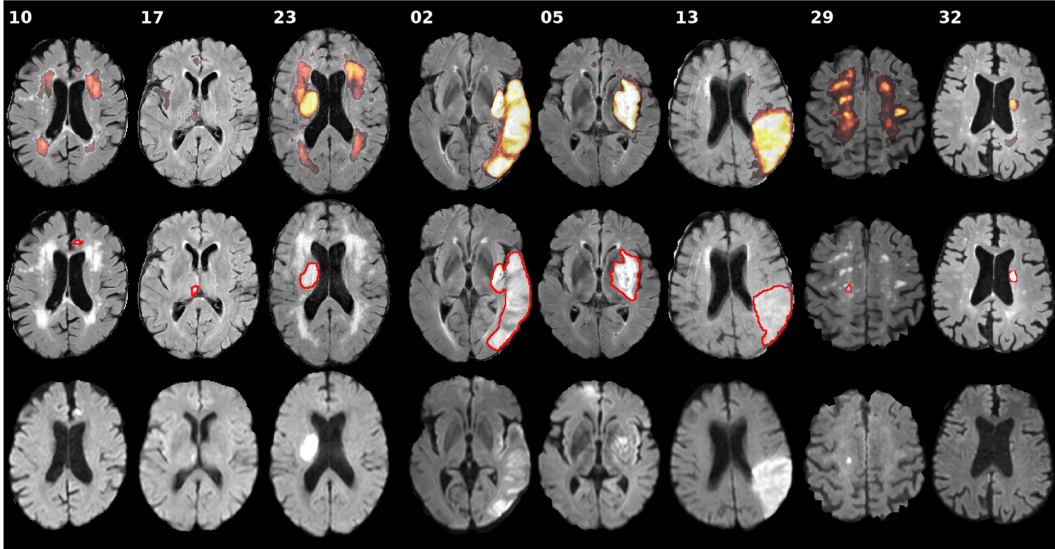
\includegraphics[width=\textwidth]{isles2015}
	\caption{Příklady snímků a výsledků z SISS. První řádek zobrazuje distribuci segmentace navržených metod na sekvenci FLAIR, druhý řádek zobrazuje stejný snímek segmentovaný expertem a na třetím řádku se nachází odpovídající DWI sekvence.}
\end{figure}
\begin{table}[]
	\label{siss results}
	\centering
	\begin{tabular}{cllll}
		\textbf{Method} & \multicolumn{1}{c}{\textbf{Cases}} & \multicolumn{1}{c}{\textbf{ASSD (mm)}} & \multicolumn{1}{c}{\textbf{DC {[}0,1{]}}} & \multicolumn{1}{c}{\textbf{HD (mm)}} \\ \hline
		UK-Imp2         & 34/36                              & 05.96 $\pm$ 09.38                         & 0.59 $\pm$ 0.31                              & 37.88 $\pm$ 30.06                       \\ \hline
		CN-Neu          & 32/36                              & 03.27 $\pm$ 03.62                         & 0.55 $\pm$ 0.30                              & 19.78 $\pm$ 15.65                       \\ \hline
		FI-Hus          & 31/36                              & 08.05 $\pm$ 09.57                         & 0.47 $\pm$ 0.32                              & 40.23 $\pm$ 33.17                       \\ \hline
		US-Odu          & 33/36                              & 06.24 $\pm$ 05.21                         & 0.43 $\pm$ 0.27                              & 41.76 $\pm$ 25.11                       \\ \hline
		BE-Kul2         & 33/36                              & 11.27 $\pm$ 10.17                         & 0.43 $\pm$ 0.30                              & 60.79 $\pm$ 31.14                       \\ \hline
		DE-UzL          & 31/36                              & 10.21 $\pm$ 09.44                         & 0.42 $\pm$ 0.33                              & 49.17 $\pm$ 29.6                        \\ \hline
		US-Jhu          & 33/36                              & 11.54 $\pm$ 11.14                         & 0.42 $\pm$ 0.32                              & 62.43 $\pm$ 28.64                       \\ \hline
		UK-Imp1         & 34/36                              & 11.71 $\pm$ 10.12                         & 0.44 $\pm$ 0.30                              & 70.61 $\pm$ 24.59                       \\ \hline
		CA-USher        & 27/36                              & 09.25 $\pm$ 09.79                         & 0.35 $\pm$ 0.32                              & 44.91 $\pm$ 32.53                       \\ \hline
		BE-Kull         & 30/36                              & 12.24 $\pm$ 13.49                         & 0.37 $\pm$ 0.33                              & 58.65 $\pm$ 29.99                       \\ \hline
		CA-McGill       & 31/36                              & 11.04 $\pm$ 13.68                         & 0.32 $\pm$ 0.26                              & 40.42 $\pm$ 26.98                       \\ \hline
		SE-Cth          & 30/36                              & 10.00 $\pm$ 06.61                         & 0.38 $\pm$ 0.28                              & 72.16 $\pm$ 17.32                       \\ \hline
		DE-Dkfz         & 35/36                              & 14.20 $\pm$ 10.41                         & 0.33 $\pm$ 0.28                              & 77.95 $\pm$ 22.13                       \\ \hline
		TW-Ntust        & 15/36                              & 07.59 $\pm$ 06.24                         & 0.16 $\pm$ 0.26                              & 38.54 $\pm$ 20.36                       \\ \hline
		Inter-observer  & 34/36                              & 02.02 $\pm$ 02.17                         & 0.70 $\pm$ 0.20                              & 15.46 $\pm$ 13.56                       \\ \hline
	\end{tabular}
	\caption{Výsledky jednotlivých týmů na ISLES 2015 pro SISS.}
\end{table}

Autoři článku uvádí, že nejsou schopni jasně rozhodnout o rozdílech ve výkonnosti navržených metod - a to ani v typech jednotlivých přístupů. Dvě nejlépe hodnocené metody, vykazovali statisticky stejnou přesnost: metoda UK-Imp2 používala hluboké učení - konkrétně \alert{neuronové konvoluční sítě}, metoda CN-Neu byla založená na fuzzy C-means. Další metody byly založené na náhodných lesech (\alert{Random Forest}). Přesto nelze říci, že by nějaká z nich pracovala výrazně lépe. Autoři zmiňují, že klíčem k úspěchu je spíše odladění hyperparametrů modelu a jeho adaptace. Nejlepší tři řešení využívali kombinaci dvou různých algoritmů, aby vykompenzovali slabá místa každého z nich.

Metody soutěžících byly rovněž otestovány na datech z jiných zdravotnických center. Zajímavým výstupem soutěže je zjištění, že ani jeden z algoritmů nebyl schopen dobře fungovat na cizích datech. Přestože metody vykazovaly dobrou generalizaci na testovacích datech pořízených ze stejného datacentra jako data trénovací.

Obecně automatická segmentace fungovala dobře na velkých lézích se silným FLAIR signálem, naopak byl problém v segmentaci malých lézí se slabým FLAIR signálem. Skóre, jaké získali soutěžící, významně korelovalo s DC. 

Článek hodnotí SISS jako velmi obtížnou úlohu - nejen na základě přesnosti navržených metod, ale i na velkém rozptylu DC napříč experty. Podle autorů by kliničtí výzkumníci neměli očekávat spolehlivé a plně automatické řešení v blízké budoucnosti, jelikož je úloha příliš složitá. Automatické segmentační algoritmy by měly sloužit spíše jako podpůrný nástroj pro radiology.

Soutěž ukázala, že aktuální stav automatické segmentace sub-akutní léze postrádá jak přesnost, tak robustnost, která je potřebná pro reálné nasazení. Dalším zjištěním bylo, že žádný z algoritmů nefungoval významně lépe proti ostatním. 

Pro budoucí výzkum autoři doporučují kombinovat různé algoritmy pro vylepšení segmentace. Evaluace by nikdy neměla být prováděna pouze na privátním datasetu a měl by být kladen důraz na adaptaci algoritmů na data z jiných center.

\subsection{Přehledové studie}

\section{Dataset}
\begin{itemize}
	\item FLAIR vs DWI
	\item Nifty - popis, registrace
	\item Možnosti rozšíření datasetu (stažení dalších dat, augmentace)
\end{itemize}

\section{Manuální segmentace}
popsat aktuální proces segmentace experta

\section{Architektury neuronových sítí}
\begin{itemize}
	\item ISLES
	\item 2D vs 3D segmentace
\end{itemize}

\printbibliography

\end{document}
